\chapter{Hessian signatures of the multistream field}
\label{appendix:Eigen}

Second-order local variations of a scalar field $f$ is described by a Hessian matrix, whose element in a three-dimensional domain is given by \autoref{eq:Hess}. The geometry of the scalar field is classified by the Eigenvalues of the Hessian. The convex regions have at-most one maxima within the (3+1)-dimensional functional space. Projection of this closed region onto three-dimensional coordinate space also gives a closed surface in coordinate space. An illustration of the projection is shown in \autoref{fig:check1d} for a simpler function $f(x)$ in one-dimensional domain. The eigenvalue criteria for regions are simplified: for instance, $\frac{\partial^2 f}{\partial x^2} < 0$ for convex region. Projection of these regions onto coordinate space is shown in the shaded regions. This is different from regions within a contour, which is the projection of the curve along which the function has a constant value. Boundaries of these two regions may, but not necessarily, intersect. 

In the case of cosmic fields, thresholds like $\Delta_{vir}$ are equivalent to the green dotted line in \autoref{fig:check1d}. The over-dense regions (green shaded regions) are not constrained to be convex. Similarly structures selected based on $n_{str}$ thresholds do not universally result in convex structures either. Local geometry can be probed from the eigenvalue criteria instead, as shown by the red line on the curve and corresponding shaded area. The projected structures, albeit convex, may have very small values of $f(x)$ (like the red shaded area around $x=5$). In the framework of identifying potential haloes in multistream field, multistream thresholds are devised in so that some of these small peaks detected by the Hessian are not considered as potential halo sites.

\begin{figure}
\begin{minipage}[t]{.99\linewidth}
  \centering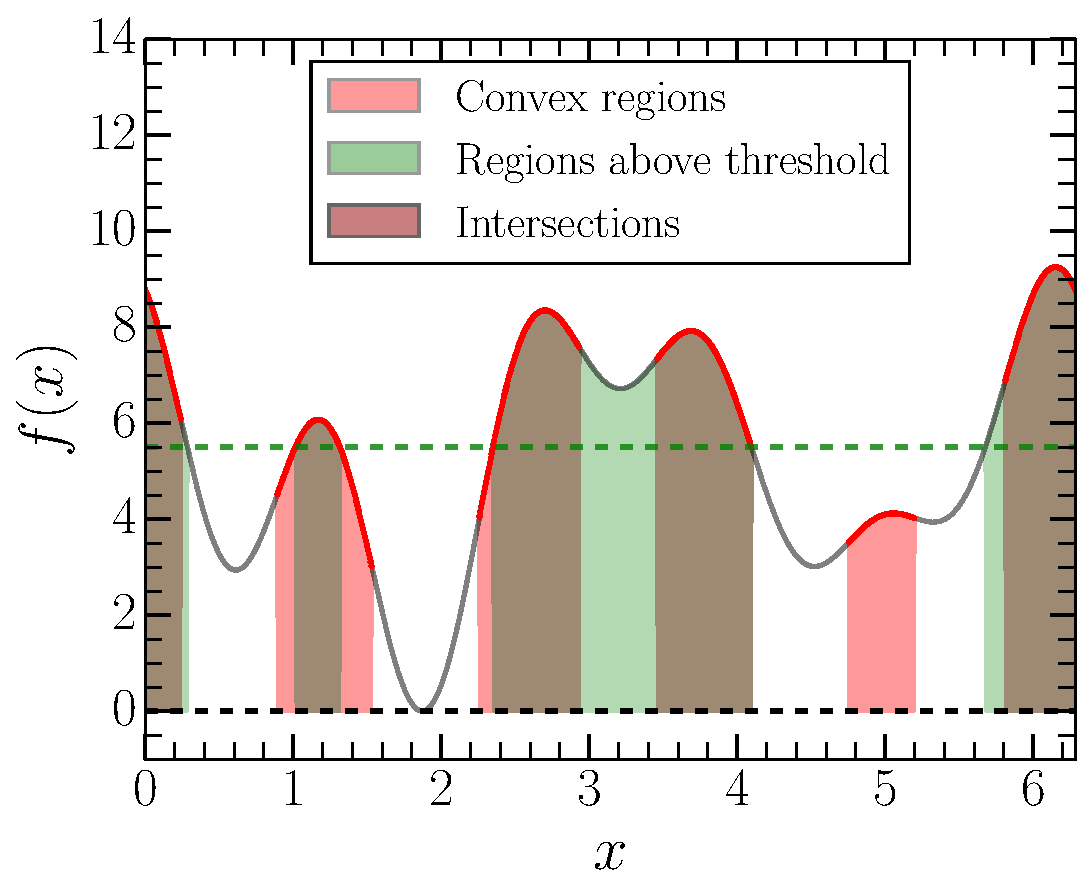
\includegraphics[width=8.cm]{Chapter5/Source_v2/fig15.pdf} 
\end{minipage}\hfill
\caption{Projections of regions of $f(x)$ from (1+1)-dimensional function space onto one-dimensional coordinate space. Convex regions and regions above a threshold of an arbitrary function $f(x)$ are shown. Both the regions intersect around a few maxima, but not universally.}
\label{fig:check1d}
\end{figure}